\chapter{Тестирование}

\section{Структура данных для дерева разбора}
Для проверки того, что код корректно преобразуется в дерево разбора, а потом обратно в исходный код, а также
для проверки достаточного покрытия программ олимпиадного программирования реализованным подмножеством языка,
были взяты случайные решения из архива \texttt{PCMS2}~--- тестирующая система, используемая в Университете ИТМО
для обучения школьников и студентов, а также проведения различных соревнований вплоть до Всероссийской командной
олимпиады школьников по программированию и полуфиналу чемпионата мира по программированию ACM ICPC.

На 47 из 50 выбранных программ структура отработала корректно. В остальных трех сказалась неполнота подмножества языка:
\begin{enumerate}
    \item В первой программе использовалось объявление типа через \texttt{record}.
    \item Во второй условный оператор \texttt{case}.
    \item В третьей конструкция \texttt{writeln(a:5:1)}.
\end{enumerate}
Все три причины не входят в подмножество языка, однако при добавлении их в грамматику, в дальнейшем смогут обрабатываться корректно.
Третья конструкция и вовсе не предусмотрена стандартной грамматикой языка Паскаль, реализованной разработчиками ANTLR, но вполне
может быть дописана на языке ANTLR, как отмечалось ранее, в грамматику можно дописать все, что душе угодно.

\section{Придуманные тесты}
\subsection{Различные популярные ошибки}
Для первоначальной проверки работы были взяты случайные решения из архива \texttt{PCMS2}, в которые были добавлены ошибки взятые из
опыта работы в учебной сфере автора работы:
\begin{itemize}
    \item Неправильные константы (Рисунок~\ref{figConst}).
        \begin{figure}[!h]
\ffigbox{
  \begin{subfloatrow}[2]
     \ffigbox[\FBwidth]{\caption{Исправление}}{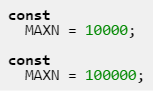
\includegraphics[scale=0.5]{pics/consts.png}}
     \ffigbox[\FBwidth]{\caption{Примененное исправление}}{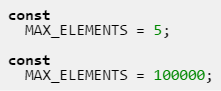
\includegraphics[scale=0.5]{pics/consts_new.png}}
  \end{subfloatrow}
}
{\caption{Исправление неправильных констант}\label{figConst}}
\end{figure}

    \item Потерянные $\pm 1$ в индексах массивов (Рисунок~\ref{figInd}).
    
    \begin{figure}[!h]
\ffigbox{
  \begin{subfloatrow}[2]
     \ffigbox[\FBwidth]{\caption{Исправление}}{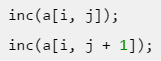
\includegraphics[scale=0.5]{pics/ind.png}}
     \ffigbox[\FBwidth]{\caption{Примененное исправление}}{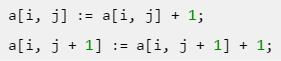
\includegraphics[scale=0.5]{pics/ind_new.png}}
  \end{subfloatrow}
}
{\caption{Исправление потерянной $+1$}\label{figInd}}
\end{figure}

    \item Неправильные типы переменных (Рисунок~\ref{figTypes}).
    \begin{figure}[!h]
\ffigbox{
  \begin{subfloatrow}[2]
     \ffigbox[\FBwidth]{\caption{Исправление}}{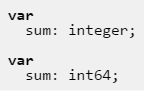
\includegraphics[scale=0.5]{pics/types.png}}
     \ffigbox[\FBwidth]{\caption{Примененное исправление}}{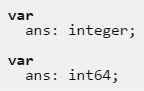
\includegraphics[scale=0.5]{pics/types_new.png}}
  \end{subfloatrow}
}
{\caption{Исправление типа переменной}\label{figTypes}}
\end{figure}

    \item Неправильные размерности массивов (Рисунок~\ref{figSize}).
    \begin{figure}[!h]
\ffigbox{
  \begin{subfloatrow}[2]
     \ffigbox[\FBwidth]{\caption{Исправление}}{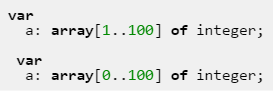
\includegraphics[scale=0.5]{pics/arrays.png}}
     \ffigbox[\FBwidth]{\caption{Примененное исправление}}{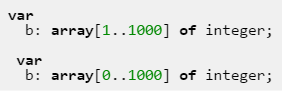
\includegraphics[scale=0.5]{pics/arrays_new.png}}
  \end{subfloatrow}
}
{\caption{Исправление размерности массива}\label{figSize}}
\end{figure}

    \item Орфографические ошибки в модификаторах, например, написать \texttt{vor} вместо \texttt{var}.
\end{itemize} 

В случае с индексами и размерностями массивов, многомерность не играет роли.

Для всех этих случаев, все работало безотказно. Однако, это сомнительный показатель, так как все-таки исправление, которое ищется
в той же самой программе. Именно поэтому перед тестами на реальных данных будет приведено последнее внутреннее тестирование. 
\subsection{Обфускация}
\textbf{Обфускация} (от англ. obfuscate~--- делать неочевидным, запутанным, сбивать с толку)~--- приведение исходного текста 
программы к виду, сохраняющему её функциональность, но затрудняющему анализ, понимание алгоритмов работы и модификацию кода. 
В промышленности данный прием применяют, например, для сокрытия корпоративных тайн, в случае, когда надо выложить код в открытый
доступ, либо для уменьшения размера кода~\cite{obfuscation}.

Одно из применений обфускации, по сути, это <<загрязнение кода>>: переименование переменных, добавление нейтральных строк, изменение форматирования
и т.д. Модифицируем предыдущий метод тестирования, применив обфускацию, которая:
\begin{itemize}
    \item переименовывает переменные в строки из десяти и больше случайных латинских букв;
    \item убирает отступы;
    \item случайно переставляет объявление функций, констант и переменных между собой;
    \item добавляет лишние переменные и константы;
    \item добавляет нейтральные строки, вида присвоения переменной, которой раньше не было какого-то значения.
\end{itemize} 

После обфускации запускаем реализованный алгоритм, затем выясняется, что он работает абсолютно также как и  в предыдущем случае.
То есть он находит исправления в таком же коде, реализованном по-другому, игнорируя другие имена переменных и изменения общей структуры.
Данный результат был довольно предсказуем, исходя из описания алгоритма, однако, тот факт, что работа оправдывает 
возложенные ожидания, не может не радовать.

\begin{figure}[!h]
\ffigbox{
  \begin{subfloatrow}[2]
     \ffigbox[\FBwidth]{\caption{Изначальное решение}}{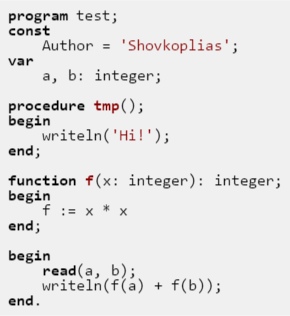
\includegraphics[scale=0.4]{pics/test.png}}
     \ffigbox[\FBwidth]{\caption{Обфускация решения}}{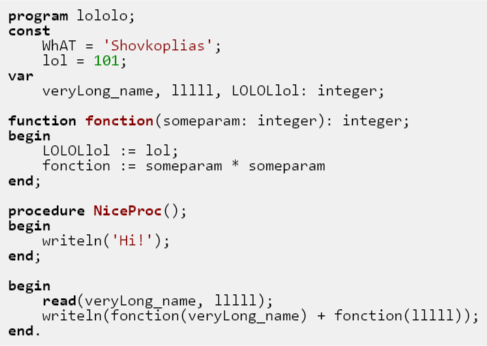
\includegraphics[scale=0.4]{pics/obfus.png}}
  \end{subfloatrow}
  
  \begin{subfloatrow}[2]
     \ffigbox[\FBwidth]{\caption{Исправленное решение}}{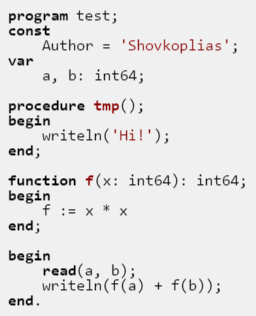
\includegraphics[scale=0.4]{pics/test_new.png}} 
     \ffigbox[\FBwidth]{\caption{Результат работы метода}}{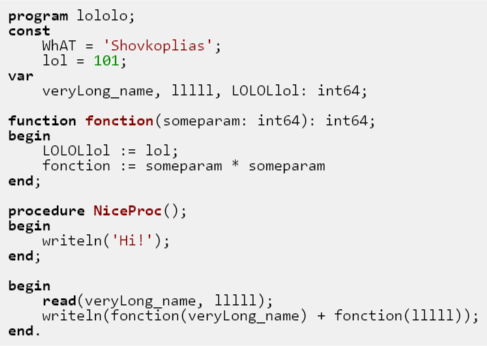
\includegraphics[scale=0.4]{pics/obfus_new.png}} 
  \end{subfloatrow}
}
{\caption{Пример работы на обфусцированных данных}\label{figO}}
\end{figure}

На рисунке~\ref{figO}, предсталена работа метода при применении обфускации к исходному решению. В данном примере, для
возможности визуального восприятия данных обфускация проведена вручную. Как видно, несмотря на изменения в тексте решения
метод нашел все переменные типа \texttt{integer}, а затем поменял их тип на \texttt{int64}.

\section{Реальные данные}

\subsection{Анализ исходных данных}

Для тестирования метода на реальных программах написанных школьниками были рассмотрены все решения муниципального
этапа Всероссийской олимпиады школьников по программированию~\cite{municipal}.

Количество участников рассмотренной олимпиады, использовавшее для написания решений язык Pascal~--- $440$ человек, и суммарно
они отправили на проверку в тестирующую систему $1865$ решений. Участникам было дано на выбор пять задач, различной сложности,
пронумерованных буквами латинского алфавита от \texttt{A} до \texttt{E}.

При описании метода в предыдущей главе задача и тест, исправления для которых мы искали, были приняты константой, однако
на реальной олимпиаде, очевидно, что пар вида задача-тест, по которым существует хотя бы одно решение <<дошедшее>> в данной задаче
до данного теста, может быть относительно много. Под <<дойти>> до теста подразумевается, что решение корректно работает на всех 
предыдущих тестах, но некорректно работает на текущем, либо текущий тест последний. В рассмотренной олимпиаде таких пар ровно
$69$.

Довольно логично, что обучаться можно только на тех решениях, для которых существует решение от того же участника, хронологически
позже отправленное на проверку, но с лучшим вердиктом.
Для каждой пары было посчитано, сколько уникальных участников получали вердикт на данном тесте по данной задаче и сколько решений 
можно использовать для обучения. В случае, если участник получал вердикт на одном и том же тесте несколько раз, бралась
последняя в хронологическом порядке посылка, а остальные игнорировались.

Далее было замечено, что тесты, которые идут в начале, не способствуют обучению, так как в большинстве своем решения, проходящие
только их, представляют из себя разбор случаев и даже близко не напоминают итоговое решение данной задачи. Для визуализации данного эффекта
для каждой задачи, для каждого теста было посчитано среднее текстовое изменение для перехода на более хороший вердикт 
(Рисунки~\ref{fig2} и~\ref{fig3}). Особенно явно этот эффект заметен в задачах \texttt{A} и \texttt{C}. В \texttt{C} это обусловлено
тем, что ответы на маленькие по размеру тесты, можно было вычислить без написания программы, а затем просто вывести.  
 
Под текстовым изменением подразумевается результат применения к двум текстам решений утилиты \texttt{diff}, которая
в результате возвращает строки, которые были изменены или удалены, а также новые строки и те, на которые измененные были заменены.
Средним текстовым изменением будет суммарный результат данной утилиты по всем решениям, поделенный на их количество.

\begin{figure}[!h] 
\caption{Диаграммы размера среднего текстового изменения по номеру теста для задач A, B, D и E}\label{fig2} 
\centering
\begin{tabular}{c c}

\scalebox{0.8}{
\begin{tikzpicture}
    \begin{axis}[
        title = A,
        %width=300,
        %xlabel = Test number,
        ylabel = Average diff,
        ybar stacked, 
        symbolic x coords={1,2,3,4,5,8,9},
        xtick=data,
        ]
        \addplot table {../graph/gr0.csv};
    \end{axis}
\end{tikzpicture}}

&
\scalebox{0.8}{
\begin{tikzpicture}
    \begin{axis}[
        title = B,
        %width=300,
        %xlabel = Test number,
        %ylabel = Average diff,
        ybar stacked, 
        symbolic x coords={1,2,7,8,10,16,17,19},
        xtick=data,
        ]
        \addplot table {../graph/gr1.csv};
    \end{axis}
\end{tikzpicture} }

\\



\scalebox{0.8}{

\begin{tikzpicture}
    \begin{axis}[
        title = D,
        %width=300,
        xlabel = Test number,
        ylabel = Average diff,
        ybar stacked, 
        symbolic x coords={1,2,3,4,6,14,29,46},
        xtick=data,
        ]
        \addplot table {../graph/gr3.csv};
    \end{axis}
\end{tikzpicture}}

&

\scalebox{0.8}{
\begin{tikzpicture}
    \begin{axis}[
        title = E,
        %width=300,
        xlabel = Test number,
        %ylabel = Average diff,
        ybar stacked, 
        symbolic x coords={1,2,3,5,8,22},
        xtick=data,
        ]
        \addplot table {../graph/gr4.csv};
    \end{axis}
\end{tikzpicture}
}

\\
\end{tabular}

\end{figure}

\begin{figure}[!h] 
\caption{Диаграмма размера среднего текстового изменения по номеру теста для задачи C}\label{fig3} 
\centering
\begin{tikzpicture}
    \begin{axis}[
        %title = C,
        width=300, 
        xlabel = Test number,
        ylabel = Average diff,
        ybar stacked, 
        symbolic x coords={1,2,3,4,5,6,7,8,10,11,15,17,20},
        xtick=data,
        ]
        \addplot table {../graph/gr2.csv};
    \end{axis}
\end{tikzpicture}

\end{figure}

Тем не менее, на долю начальных тестов, а также последних тестов, которые характеризуют успешную сдачу задачи пришлось подавляющее
большинство рассмотренных решений. Чтобы иметь хоть какую-то репрезентативность, было принято решение рассматривать только такие пары
задача-тест, где количество решений, на которых можно обучиться хотя бы пять, а также средний размер текстового изменения относительно
мал.

Под выбранное условие подошли:
\begin{itemize}
    \item Тест 8 в задаче \texttt{B}
    \item Тест 17 в задаче \texttt{C}
    \item Тест 6 в задаче \texttt{D}
\end{itemize}

\subsection{Непосредственное тестирование и полученные результаты}

Процесс тестирования проходил следующим образом:
\begin{enumerate}
\item Программа реализующая предложенный метод выбирала на решения, которые можно было бы использовать для обучения.
    Как правило, не во всех решениях были именно <<мелкие>> ошибки, однако, остальные игнорировались.
\item Затем программа перебирала одно решение из выбранных, чтобы обучиться на остальных и посмотреть: возможно ли будет
    исправить выбранное.
\item За результат было взято количество выбранных решений, которые получилось исправить, основываясь на опыте, полученном
    при рассмотрении остальных задач из выборки.
\item Также были рассмотрены решения, у которых не было решений от того же участника, хронологически
    позже отправленных на проверку, но с лучшим вердиктом. Для каждого из них пробовалось применить хотя бы одно исправление из опыта,
    чтобы улучшить вердикт.  
\end{enumerate}
Результаты представлены в таблице~\ref{tab1}.

\begin{table}[!h]
\caption{Таблица результатов тестирования}\label{tab1}
\centering
\pgfplotstabletypeset[
    col sep=&,
    row sep=\\,
    every head row/.style={
        before row=\toprule,after row=\midrule},
    every last row/.style={
        after row=\bottomrule},
    columns/Задача/.style={string type,column type=c},
]{
Задача & Тест & Всего & Пары для обучения & Результаты & Дополнительно \\
B  & 8  & 20 & 5  & 2 & 1 \\
C  & 17 & 27 & 12 & 11 & 5 \\
D  & 6  & 30 & 6  & 2 & 0 \\
}
\end{table}

Данные результаты показывают, что даже при низкой репрезентативности решений для обучения, ошибки повторяются и возможно применение
исправлений. А в случае, если репрезентативность выше, как в паре $(C;17)$, то результаты будут улучшаться.

В приложении~\ref{pril1}, приведен пример пары решений, использовавшихся для обучения (листинги~\ref{lstA1:apx} и~\ref{lstA2:apx}),
с последующим применением данного исправления к решению в листинге~\ref{lstA3:apx}. 
В результате получен код из листинга~\ref{lstA4:apx}. Результат при тестировании проходит все тесты.

Также было проведена попытка применить исправления известные после рассмотрения данных пар задача-тест к другим решениям, и было
найдено три решения, для которых применимо одно из исправлений, применяемое в паре $(B;8)$, а именно по одному решению для пар:
\begin{itemize}
\item $(B;7)$
\item $(B;10)$
\item $(C;6)$
\end{itemize}

В приложении~\ref{pril2}, в листингах~\ref{lstB1:apx} и~\ref{lstB2:apx}, представлены два решения дающие исправление
с $7$-го до $10$-го теста.
Однако, дальше это исправление, пробуется применить к программам из листингов~\ref{lstB3:apx} и~\ref{lstB5:apx}, в результатах
получаются программы из листингов~\ref{lstB4:apx} и~\ref{lstB6:apx}, соответственно. 

\chapterconclusion

\begin{enumerate}
    \item Проведено тестирование структуры данных.
    \item Проведено тестирование на искусственных и естественных тестах.
    \item Показаны результаты работы.
\end{enumerate}
